\chapter{Theory}
\section{Bivalve molluscs}
General description of their distribution, sessile lifestyle, ability to accumulate pollutants without high mortality, feeding strategy etc. The common blue mussel (\emph{Mytilus edulis}) is a marine bivalve residing on hard substrates of the sediment/water interphase and intertidal zones of temperate waters. It is a suspension feeder, filtering high quantities of water for suspended particulate matter (\cite{Beyer2017b}). This feeding strategy makes them highly effective in micro- and nano-scaled particle uptake, and consequently especially susceptible to engineered NP exposure (\cite{Canesi2012}). \emph{Mytilus sp.} has served as sentinel species in marine monitoring programs since the 1970s (\cite{Goldberg1975}), are highly suitable for assessing engineered NP toxicity. Bridge that leads on to their immune system and use as systems of immunotoxicity and genotoxicity.

\begin{figure}[h]
    \centering
    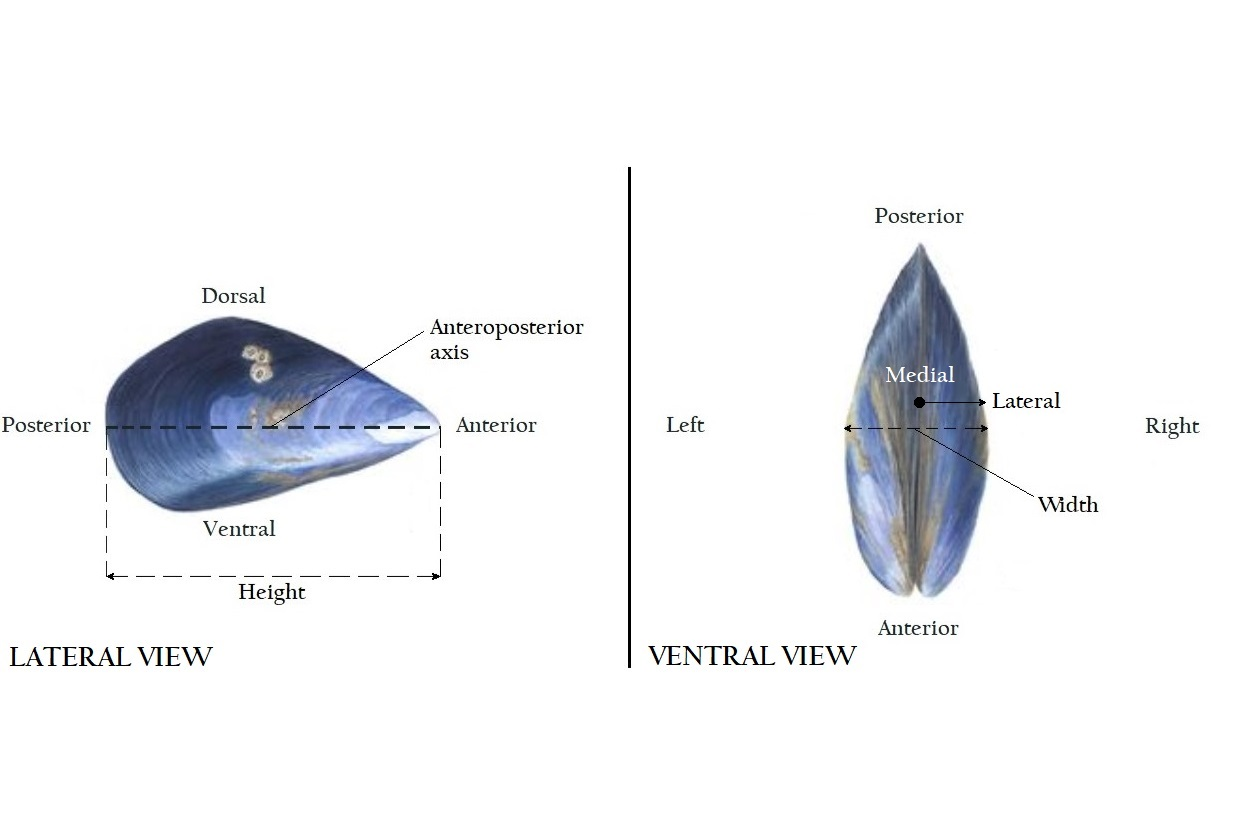
\includegraphics[width=\textwidth]{figures/Anatomy/M_edulis_anatomical_axis_lateral.jpg}
    \caption{The figure caption depends on if it ends up here, or in the material and method. Write when decided. The illustration was adapted from an artistic work by Abby Towne, A. Towne Design with permission.}
    \label{fig:anatomical_axis}
\end{figure}


\subsection{Classification of the haemocyte subpopulations of \emph{M. edulis}}
\label{subsection:haemocyte_classification}
Since the first written account on the subject (\cite{Cuenot1891}, cited in: \cite{Cheng1980}), several authors have devoted their attentions to developing a unifying classification system for the amoebocytic blood cells of bivalve mollusks, more commonly known as haemocytes (\cite{Cheng1980, delaBallina2022}). Belonging to the bivalve familiy \emph{Mytilidae}, the haemocytes of \emph{Mytilus edulis}, \emph{Mytilus galloprovincialis} and several other commercially important species of the genus \emph{Mytilus} have been encompassed by these efforts, creating a substantial pool of literature on the haemocytes of this genus alone. Despite a lack of consensus for any unifying classification system for the haemocytes of this phylum at large, the literature that exists on the haemocytes of \emph{M. edulis} generally agrees on the existence of three distinct subpopulations.

The first effort to classify the haemocytes of \emph{M. edulis} was made by Moore and Lowe (1977). Much like the other attempts to classify bivalve haemocytes at the time, this classification was based on the morphofunctional aspects of these cells - a system that has been extensively reviewed by Hine (1999). Moore and Lowe constructed a simple classification based on static morphological and ultrastructural characteristics of the haemocytes, combined with their phagocytic capacities (\cite{Moore1977}). From routine cytological staining, they identified three haemocyte subpopulations (or cell types): "(1) small basophilic hyaline cells or lymphocytes, (2) larger basophilic hemocytes with varying degrees of irregular cytoplasmic granulation and vacuolation, and (3) eosinophilic granular haemocytes or granulocytes" (\cite{Moore1977}). The small basophilic cells (4-6 \micro m) were generally spherical in outline, had a scant thin rim of basophilic hyaline (read: transparent) cytoplasm and a spherical nucleus - bearing resemblance to vertebrate lymphocytes. The larger granular basophils (7-10 \micro m) displayed less intense basophilic cytoplasm, lower nuclear:cytoplasmic (N:C) ratios and more irregularly shaped nuclei. The eosinophilic granulocytes were the largest cell type identified (7-12 \micro m). They had a regular spherical appearance, further characterized by a small round nucleus, low N:C ratio, and a cytoplasm filled with spherical eosinophilic granules (0.5-1.0 \micro m).

Electron micrographs confirmed the existence of three ultrastructurally distinct morphologies. Except for a few mitochondria, the lymphocyte-like cells contained a scarcity of organelles and granules. This stood in sharp contrast to the larger granular basophils, which contained Golgi apparatus, phagosomes and smaller granular inclusions - possibly representing primary lysosomes. A phagocytosis assay with experimentally injected carbon particles revealed that both granular cell types displayed phagocytic properties, while the small lymphocyte-like cells did not show any evidence for this capacity (\cite{Moore1977}).

The morphological and ultrastructural findings of Moore and Lowe (1977) have since been confirmed by several investigators (\cite{Rasmussen1985, Renwartz1990, Pipe1990, Noel1994, Pipe1997, Wootton2003}). From their stand-alone electron microscopical examinations, Pipe and colleagues (1990) made a distinction between granular haemocytes with small (0.2-0.3 \micro m) and large (0.5-1.5 \micro m) granules. By relating the two ultrastructural phenotypes to their cytological staining properties, investigators soon demonstrated that the two cell types corresponded to the basophilic and eosinophilic granular haemocytes of Moore and Lowe (\cite{Pipe1990, Noel1994}). Thus, if reduced to it's static morphological criteria, Moore and Lowe's classification of \emph{M. edulis} haemocytes coincides with the original system of Cúenot (1891). This system generally recognized three types of haemocytes in bivalves: "(1) finely granular haemocytes, (2) coarsely granular haemocytes and (3) cells with very little cytoplasm surrounding the nucleus" (\cite{Cheng1984}). 

Leaning towards a phylum-wide two-categorical classification (hyalinocytes and granulocytes), Cheng (1981) argued that a distinction between the basophillic and eosinophilic granulocytes of \emph{M. edulis} was artificial, as he saw them as being immature and mature stages of the same cell type (granulocytes), respectively. From observations of what resembled intermediate stages between the lymphocyte-like and larger basophilic cells, Moore and Lowe (1977) had argued that the basophilic cells constituted an ontogenic developmental series, with the larger phagocytic macrophages representing the final stage of differentiation. This was further supported by observations of lymphocyte-like cells with mitotic figures, suggesting that it could be the stem cell of this lineage (\cite{Moore1977}). Since a few smaller eosinophilic granulocytes (5-7 \micro m) were observed in their sections, the eosinophilic granulocytes were believed to represent a distinct growth series.

As noted by Cheng (1984), this theory was not based on direct evidence, but consisted mainly of interpretive evaluations of morphological findings. The classification of bivalve haemocytes should ideally be constructed on the basis of their ontogeny. However, mapping of ontogenic lineages among bivalve haemocytes have been tempered by the lack availible molecular databases, no one unifying model species, combined with uncertainty regarding the hematompoietic tissue(s) and processes of bivalves (\cite{Hine1999, Smith2016, Pila2016, delaBallina2022}). With no real ontogenic evidence to work with, a careful assessment of availible morphological data may represent a better alternative relative to a classification based solely on biochemistry and function (\cite{Hine1999}). 

\subsubsection{Flow cytometric classification haemocytes of \emph{M. edulis}}
Almost two decades after flow cytometers became commercially availible in the 1970s (\cite{Shapiro2004}), the application of these instruments started to gain traction within the field of invertebrate immunopathology (\cite{Fisher1988}). Since the traditional characterization of bivalve haemocytes were largely based on morphological criteria such as size, granularity and staining affinities, the simultaneous measurement of forward scatter (\acrshort{fsc}, $\approx$ size) and side scatter (\acrshort{ssc}, internal complexity $\approx$ granularity) represented a far less subjective approach to their characterization (\cite{AshtonAlcox1998, Allam2002, Mateo2009}).

A detailed flow cytometric characterization of the haemocytes of \emph{M. edulis} was undertaken by Le Foll and colleagues (2010), who were able to distinguish three subpopulations according to their cell diameters (\micro m) and Side Scatter (\acrshort{ssc}) (\cite{LeFoll2010}). These comprised one population of small cells (7.14$\pm{0.05}$ \micro m) with low \acrshort{ssc}, one population of larger cells (9.97$\pm{0.17}$ \micro m) with intermediate \acrshort{ssc} and one population of large cells (10.08$\pm{0.24}$ \micro m) with high \acrshort{ssc}. By running haemocytes stained with eosin - which is fluorescent in the green/yellow spectrum under blue laser exitation (\cite{Elfer2016, Koegle2020}) - they were able to identify the latter cluster as eosinophilic granulocytes. The use of flow cytometers equipped with cell sorting capabilities simplifies the process of verifying any classification derived from flow cytometric measurements (\cite{Shapiro2004}). However, when extracting cells with known measured characteristics is not possible, the cells to be classified can be separated by other means prior to flow cytometric acquisition.

Since the three haemocyte cell types of \emph{M. edulis} differ with regard to the size and density of their granules, Friebel (1995) and Pipe (1997) managed to physically separate the eosinophilic granulocytes from the two basophilic cell types by isopycnic centrifugation (\cite{Friebel1995, Pipe1997}). Depending on the fixative used, the whole haemocyte population separated into three or four distinct cell-bands in the interfaces of the various layers. The two basophillic cell types could be isolated in high purity from the upper cell band (lowest density), the eosinophilic granulocytes from the lower, while the intermediate fractions often consisted of varying proportions of all three cell types. Accompanied by the rapid growth of flow cytometric applications in invertebrate immunology, the progress made by Friebel (1995) and Pipe (1997) meant that results from functional and biochemical assays could be assigned to specific cell types at a higher throughput. Thus, the unraveling of the roles of individual haemocyte subpopulations really started to pick up speed.

\section{The role of hemocytes}
Use articles citing Friebel and Renwrantz (1995) to locate articles that have a characterized these cell-types in therms of enzyme activity and cytochemistry. (E.g. 10.1016/j.jip.2009.10.001).

Functional classification based on phagocytic capacity: Differences in phagocytosis between granulocytes and agranular haemocytes may be related to the type of phagocytosed particles involved, rather than differences in phagocytic ability (Hine, 1999)

Unlike granulocytes and hyalinocytes, precursor cells do not contribute to immune-response mechanisms such as phagocytosis or encapsulation, and they also lack common intracellular enzyme systems associated with host defence. 

Their lack of cytoplasmic organelles seems to preclude a secretory or phagocytic function

Basophilic cytoplasm suggest the presence of free ribosomes and immaturity

Refer to the 1990 study of Pipe when explaining the functions of the cytoplasmic granules.

Hemocytes also (in addition to lung and digestive gland) showed high expression levels (of initiator and executioner caspases), probably due to the role of apoptosis in the defense against pathogens. Because bivalves are highly susceptible to climate changes, pollutants and pathogens, it  could be suggested that a strong apoptotic process may be necessary to ensure body homeostasis. (Romero, 2011). See page 11 of (New Insights into the Apoptotic Process in Mollusks: Characterization of Caspase Genes in Mytilus galloprovincialis) for greater detail and references.

\section{Bivalve hemocytes as \emph{in vivo} model systems for immunotoxicity}
Used as membrane integrity model system. "Since their membranes are susceptible to being destabilized by different stressors, this feature has been frequently used as a biomarker to monitor pollution and animal health (reviewed in Moore et al. 2004, 2006)." From "Changes induced by two strains of Vibrio splendidus in haemocyte subpopulations of Mya arenaria, detected by flow cytometry with LysoTracker" (Mateo, 2009), DOI: 10.3354/dao02121. The total hemocyte count (\acrshort{thc}) decreased by 66\% after a bacterial injection \cite{Parisi2008}.

\subsection{The mussel micronucleus cytome Assay}
Micronuclei (\acrshort{mni}) are small cytosolic membrane-enclosed chromatin bodies that contain acentric chromosome fragments or whole lagging chromosomes that remain outside the nucleus of daughter cells after cell division (\cite{Fenech2011}). Micronuclei with acentric fragments can originate from unrepaired or misrepaired DNA-breaks from interactions with clastogenic chemicals, while larger MNi with whole chromosomes arise from indirect interactions with the replication apparatus during anaphase (aneugenic mechanism) (\cite{Fenech2011}). While the two structures may provide mechanistic information about the tested chemical, they are not readily distinguishable in standard cytologic preparations (\cite{Natarajan1993}). Without specific labeling of kinetochores or centromere-specific DNA, mNi provide general evidence for direct or indirect genotoxic damage (\cite{Tucker1996, Lynch1993}).

These cytogenic damages are the major endpoints of micronucleus assays, which represent instrumental tests in the hazard identification of genotoxic compounds (\cite{OECD474, OECD487}). Since there is a strong association between specific cytogenic alterations and tumorigenesis, the implementation of this biomarker in toxicological risk assessment is well justified (\cite{Mitelman1983} in: \cite{Tucker1996}). Micronucleus tests are performed on dividing or newly divided cells, and are most typically used to assay genotoxic damage in cells from bone marrow samples and blood in the case of mammalian test systems (\cite{Heddle1983, Warheit2018b}).

Micronucleus tests have also been extended for use in ecotoxicology, and represent one of the most prevalent biomarkers of genotoxicity in aquatic animals (\cite{Bolognesi2012}). Bolognesi and Fenech (2012) further updated and refined the existing MN test for bivalve haemocytes and gill cells to include scoring of necrotic and apoptotic cells as endpoints for cytotoxicity, by following the cytome approach applied in mammalian cells (\cite{Fenech2007} in: \cite{Bolognesi2012}). Scoring of cells with nuclear buds (NBUDs) were also included as a biomarker of elimination of amplified DNA and/or DNA repair complexes, although the mechanism leading to NBUD formation is not completely known (\cite{Bolognesi2012}).

The Mussel MN cytome protocol proposed scoring of MNi in agranular haemocytes, which were characterized by their small size (3-4 \micro m), high N:C ratio and lack or low abundance of cytoplasmic granules and organelles (\cite{Bolognesi2012}). This suggestion was based on the findings of Vernier et al. (1997), who reported that the "granular haemocytes" of \emph{M. galloprovincialis} were less sensitive to MN induction by Benzo[a]pyrene. However, Vernier and colleagues were not able to establish wether their "agranular haemocytes" corresponded to the basophilic granular haemocytes of Friebel and Renwrantz (1995) or lymphocyte-like cells in the original publication, but later referred to them as hyalinocytes in the work cited by Bolognesi and Fenech (2012) (\cite{Dolcetti2002}). The attached photomicrographs of micronucleated agranular haemocyte did however represent large basophilic haemocyte with cytoplasmic vacuolation (\cite{Venier1997, Dolcetti2002}), i.e., not a small agranular haemocyte (3-4 \micro m). This celltype has been described as granulocytes with small granules in \emph{M. galloprovincialis} (\cite{Carballal1997}), which are equivalent to the larger granular basophils of \emph{M. edulis} (\cite{Moore1977}).

While there are discrepancies between the proposed target cell and the underlying argumentation by Bolognesi and Fenech (2012), the proposition may still be sound in context of micronucleus formation and the current scientific understanding of bivalve hematopoiesis. The "agranular haemocytes" of Bolognesi and Fenech have many names (small hyaline, blast-like, lymphocyte-like, hemoblast-like cells, etc.), but they are all invariably describing small agranular cells with very little cytoplasm surrounding the nucleus. Since their basophilia indicates the presence of free ribosomes and immaturity, while their lack of cytoplasmic organelles precludes a secretory or phagocytic function, these cells are thought to represent the immature "prohemocyte" precursor of one or both granular cell types (\cite{Hine1999, delaBallina2022, Smith2016}). As MNi only arise in dividing cells, this likely explains why Vernier et al. (1997) found the eosinophilic granulocytes to be less sensitive targets of cytogenic damage.

However, as the small agranular haemocytes of \emph{M. edulis} (< 6\micro m) may make up as little as 2\% of the total haemocyte population (present/current work), this criteria may be unattainable or just very time-consuming in samples from such individuals.

If I argument for the scoring of basophilic cells in general, I won't need to prove that cluster 1 is blast-like cells exclusively.

Scoring a defined subpopulation of hemocytes for nuclear anomalies by light microscopy is a time-consuming and labor-intensive process... Bridge to semi-automation: inter-operator variability, subjectivity etc.

Haemolymph smears can be messy. Therefore, scoring of necrotic and apoptotic haemocytes by microscopy should be performed by certified operators with formal education or practice from hematology or immunology. A few example PNG images with from a published protocol leaves too much to subjectivity. 


\section{Cellular methods}
Short introduction to the concept of measuring cell viability, and membrane integrity and apoptosis by flow cytometry. Leads to "in this assay, necrosis and apoptosis was measure by Calcein A/ToPro3 and Apo15/ToPro3".

\subsection{Calcein AM/TO-PRO-3 Iodide viability assay} 

\acrshort{calceinam} is an electrically neutral molecule, which can easily penetrate cells through diffusion. After acetoxymethyl ester hydrolysis, the negatively charged Calcein molecules are trapped within the cell.

Calcein is a polyanionic fluorescein derivative that bears five negative charges and two positive charges at pH 7 (\cite{Wallach1959}).

It's fluorescence is fairly constant between pH 5-9 \cite{Chiu1977}.

the leading esterase substrate for viability assays (\cite{Ramirez2010})

Low toxicity: Calcein/AM induced no immediate loss (3 h) of membrane integrity (10.1097/00001813-199508000-00011).

Calcein-acetoxymethyl ester (calcein/AM) is a nonfluorescent molecule, converted by intracellular esterases into a fluorescent, cell impermeant acidic form \cite{Uggeri2000}.

Substrate of P-glycoprotein (P-gp/MDR-1): is used to test wether a compound is a P-gp inhibitor (\cite{Di2016}). When blockers inhibit the
pumping activity of P-gp, more fluorescent calcein accumulates within the cells and can be assayed by its fluorescence (\cite{Köhler2003}).
Since eosinophilic granulocytes have higher levels/activity of MDRP-1 than the basophilic cell types (\cite{Rioult2014}), calcein fluorescence can be used indirectly indirectly to assay the this cell type.




\subsection{Apo15/TO-PRO-3 Iodide apoptosis assay}
Theory behind Annexin-V/Apo-15 (\cite{Barth2020}) Annexin V has affinity for phosphatidylserine, which is externalized to the outer layer of the plasma membrane in the earlier stages of apoptosis. Annexin V also binds internal phosphatidylserine (\acrshort{ps}) in permeable membranes, i.e. dead cells. Thus, dead cells are Apo-15+ ToPro3+, while the early apoptotic cells are only Apo15+. The Annexin V/PI assay is considered the the gold standard of \emph{in vitro} apoptosis detection, but requires free Ca$^{2+}$.


\section{Objective}
